\documentclass[11pt]{article}
\newcommand{\tb}{\textbf}
\usepackage{listings}
\parindent 0in
\parskip 1em
\usepackage{graphicx}
\begin{document}
	\title{\textbf{COMPUTER ARCHITECTURE \& ASSEMBLY LANGUAGE HW4 PART 2 - Adil Hydari}}
	\maketitle
	
\section*{Problem 1 - Solution}
The decision to avoid non-taken branch predictions or delay-branch strategies in a 10-stage pipeline is affected by the pipeline's complexity and the penalties for mispredicting. In deep pipelines, the number of pipeline stages that need to be flushed due to a misprediction is greater compared to shorter pipeline, such as a 5-stage pipeline. This results in a higher cost for each misprediction since more stages have to be flushed of an instruction before proceeding and a larger flush means more clock cycles wasted. Inserting delay slots to manage delay branches adds significant complexity to the processor. This complexity comes from having to fill those delay slots with useful instructions that do not alter the behavior of the branch itself or lead to any other hazards. The deeper the pipeline, the more challenging it becomes to manage the delays efficiently without increasing the risk of errors. Intel itanium was a great example of this, it was essential (at least to me) a computer hardware designer's pipedream. A cpu that threw the whole research of the pentium and celeron era out of the window by for-going superscalar and out-of-order execution and instead heavily relied upon instruction level parallelism with a deep in-order pipeline. This meant that it was almost entirely up to the compiler to make a decision on parallel issuing of instructions, instructions must be grouped into bundles of three (bundle = 128 bits), and can read up to two bundles per clock from the L1 cache into the pipeline. Itanium completely flopped however, though being what many today consider the ideal RISC implementation of a pipeline; in the end, the complexity of putting the burden of the parallelism on the compiler was too great for gcc or even intel to overcome. Even a year or so after the launch of itanium the compiler was dreadfully behind, in many cases it could not even fully saturate all parallel lanes of the processor. Each instruction was 42.6 bits long, wasting an awful amount of time trying to saturate data from the data memory or instruction memory into the pipeline, further, various types of hazards could not be solved dynamically at run time, and instead had to be handled by the compiler with stalls, which added even more complexity on top of a already deep, complex pipeline. Even more than that,  itanium was just flat-out expensive, even when intel had worked out all the issues with the hardware architecture and compiler, itanium was almost exclusively a enterprise product, albeit one that provided massive scalability and massive improvements in streaming instructions. At its heart, itanium was still a In-order type processor, which meant that the amount of ILP that could be extracted from the processor was minimized, even if speculation on the IA-64 architecture was quite advanced. \\

Advanced branch prediction mechanisms increase both the development cost of processors and their final market price. This could make high-performance processors less accessible for budget-constrained settings such as schools or startups, limiting access HPC resources. 

\section*{Problem 2 - Solution}
Traditional: 1 instruction per cycle, 6 instructions per iteration = 6 cycles.
Speedup: 6 (traditional)/32 (non-forwarding)=0.187532 (non-forwarding) (not actually a speedup; the pipelined version is slower due to stalls).

5-Stage with Forwarding, Predict Taken vs. Traditional:
Speedup: 6(traditional)/30 (with forwarding, taken) = 0.230 (with forwarding, taken)

5-Stage with Forwarding, Predict Taken vs. 5-Stage Non-Forwarding:
Speedup: 32 (non-forwarding)/30 (with forwarding, taken)=1.06730 (with forwarding, taken).

5-Stage with Forwarding, Predict Not Taken vs. Traditional:
Speedup: 6(traditional)/30 (with forwarding, not taken)=0.230 (with forwarding, not taken)

5-Stage with Forwarding, Predict Not Taken vs. 5-Stage Non-Forwarding:
Speedup: 32 (non-forwarding)/30 (with forwarding, not taken)=1.06730 (with forwarding, not taken)

10-Stage with Forwarding, Predict Taken vs. Traditional:
Speedup: 6 (traditional)/60 (10-stage, taken)=0.11552 (10-stage, taken)

10-Stage with Forwarding, Predict Taken vs. 5-Stage Non-Forwarding:
Speedup: 32 (non-forwarding)/60 (10-stage, taken)=0.61552 (10-stage, taken)

10-Stage with Forwarding, Predict Taken vs. 5-Stage with Forwarding, Predict Taken:
Speedup: 30 (5-stage, taken)/60 (10-stage, taken)=0.57752 (10-stage, taken)

10-Stage with Forwarding, Predict Taken vs. 5-Stage with Forwarding, Predict Not Taken:
Speedup: 30 (5-stage, not taken)/60 (10-stage, taken)=0.57752 (10-stage, taken)

I have done the calculations, but instead of just the calculations I have something else that is pretty cool. I have 2 implementations of a RISC-V processor in verilog, one is a 5-stage with a stall unit, and the other is a 5-stage with forwarding and branch prediction in the form of GShare and PShare. 
\\
\begin{figure}
	\centering
	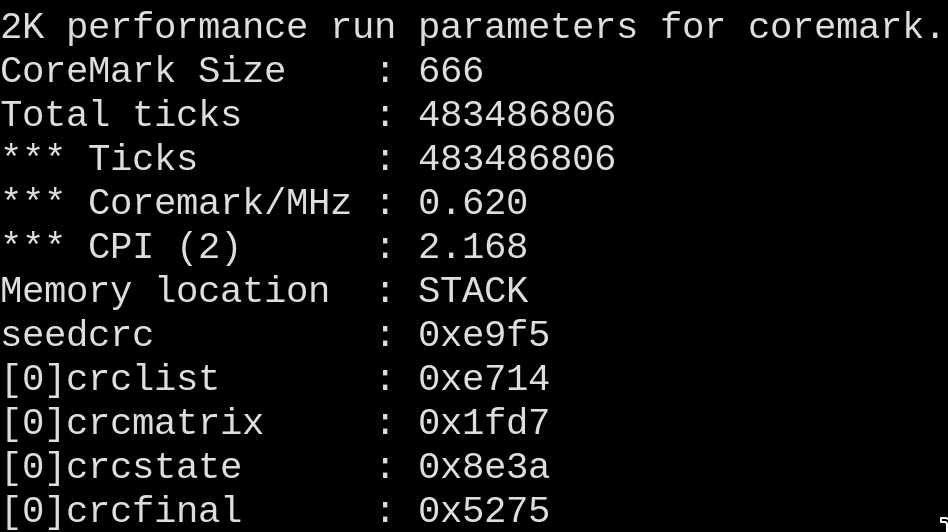
\includegraphics[width=0.7\linewidth]{screenshot001}
	\caption{Working example of a 5 stage processor with bubbles (Coremark).}
	\label{fig:screenshot001}
\end{figure}
\begin{figure}
	\centering
	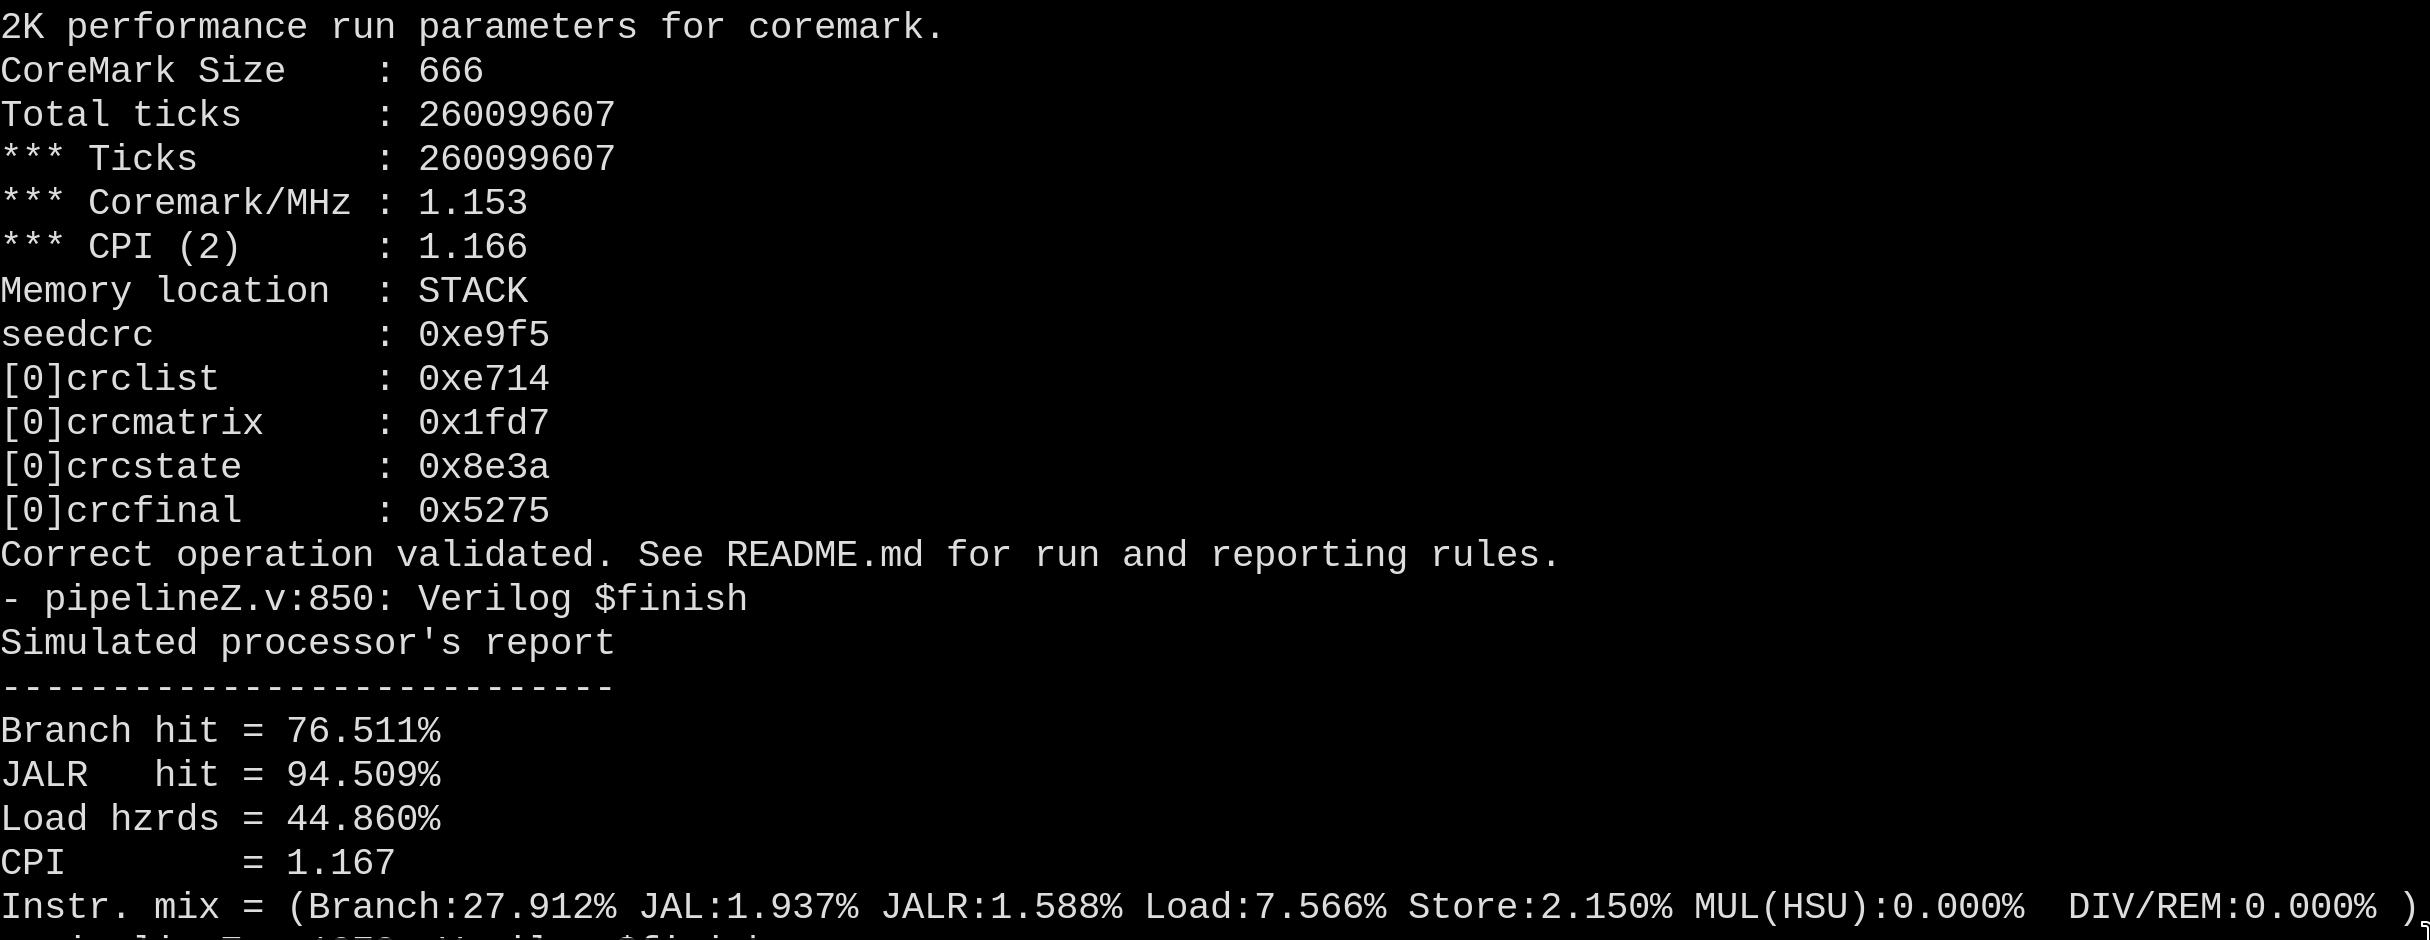
\includegraphics[width=0.7\linewidth]{screenshot002}
	\caption{Working example of a 5 stage processor with forwarding, branch support, and branch prediction (Coremark)}
	\label{fig:screenshot002}
\end{figure}
\subsection*{Cost vs. Speedup Analysis}

\textbf{5-stage non-forwarding (\$4,000) vs. traditional (\$2,000):} The doubling in speed might be justifiable in environments where doubling the performance leads to significantly enhanced capability, considering the cost is doubled.\\
\textbf{5-stage with forwarding (\$7,000) vs. traditional:} This setup offers a higher speedup, but the cost is 3.5 times higher. This might be suitable for applications where faster data processing has a dramatic impact, like real-time systems or HF trading.\\
\textbf{10-stage with forwarding (\$12,000) vs. traditional:} The highest speedup, but also the highest cost. This might be justified in environments like scientific research or simulation where small increments in processing speed can save time in the long run.\\

\subsection*{Applications of processors}
\textbf{General Computing vs. Specialized Tasks:} For everyday computing tasks, such as web browsing, the cost of advanced processors does not translate into noticeable benefits for the end user. On the other hand, for data-intensive fields like CFD or ASIC simulation, even small performance gains could be crucial, justifying higher costs.


	
\end{document}